\chapter{Introduction}
\newlecture{Sergio Savaresi}{16/04/2020}

\section{General topics of MIDA course}

\begin{itemize}
    \item Collect digitally data from real systems
    \item Build black-box (gray-box) models from data, with emphasis on
    \begin{itemize}
        \item Dynamic systems
        \item Control/automation-oriented applications
    \end{itemize}
    \item Purpose of modelling (area of machine leasing focusing on ``control'')
    \begin{itemize}
        \item Prediction
        \item Software-sensing
        \item Modelling for control design
    \end{itemize}
\end{itemize}

\subsection{Super summary of MIDA 1}
The focus is on \emph{time series} (output-only systems) and \emph{input/output} (I/O) systems.

Models used in MIDA1:
\begin{itemize}
    \item ARMA models for T.S.
    \item ARMAX models for I/O systems
\end{itemize}

\begin{figure}[H]
    \begin{minipage}[t]{0.4\textwidth}
        \centering
        \begin{tikzpicture}[node distance=2.5cm,auto,>=latex']
            \node [int] (a) {$\frac{C(z)}{A(z)}$};
            \node (b) [left of=a, node distance=2cm] {};
            \node (end) [right of=a, node distance=2cm]{};
            \draw[->] (b) edge node {$e(t)$} (a);
            \draw[->] (a) edge node {$y(t)$} (end);
        \end{tikzpicture}
        \caption*{ARMA model}
    \end{minipage}
    \begin{minipage}[t]{0.4\textwidth}
        \centering
        \begin{tikzpicture}[node distance=2.5cm,auto,>=latex']
            \node [int] (a) {$z^{-k}\frac{B(z)}{A(z)}$};
            \node (b) [left of=a, node distance=2cm] {};
            \node [sum] (c) [right of=a, node distance=2cm] {};
            \node [int] (d) [above of=c, node distance=1.5cm] {$\frac{C(z)}{A(z)}$};
            \node (e) [left of=d, node distance=2cm] {};
            \node (end) [right of=c, node distance=2cm]{};
            \draw[->] (b) edge node {$u(t)$} (a);
            \draw[->] (e) edge node {$e(t)$} (d);
            \draw[->] (a) edge node[pos=0.8] {$+$} (c);
            \draw[->] (d) edge node[pos=0.8] {$+$} (c);
            \draw[->] (c) edge node {$y(t)$} (end);
        \end{tikzpicture}
        \caption*{ARMAX model}
    \end{minipage}
\end{figure}

The model is indicated as $\mathcal{M}(\theta)$ where $\theta$ is the parameter vector, the coefficients of $A(z)$, $B(z)$, $C(z)$.

A \textbf{parametric identification method} has been used: the \emph{performance index is defined}
\begin{definition}
    $J(\theta) = \frac{1}{N} \sum_{t=1}^N \left(y(t) - \hat{y}(t|t-1, \theta)\right)^2$
\end{definition}

Which is the variance of the \emph{prediction error} made by the model. The optimal $\theta$ is $\hat{\theta}_N = \argmin_\theta J(\theta)$

\subsection{MIDA 2}

The focus is on I/O systems (more close to real applications than T.S.).

\begin{description}
    \item[Chapter 1] non-parametric (direct/constructive) black-box identification of I/O systems using state-space models
    \item[Chapter 2] parametric identification fo black-box I/O systems, with a frequency-domain approach
    \item[Chapter 3] Kalman-filter for Sw-sensing using feedback on white-box models
    \item[Chapter 4] black-box methods for SW-sensing without feedback
    \item[Chapter 5] gray-box system identification using Kalman-filter and using \emph{simulation-error methods} (S.E.M,)
    \item[Chapter 6] Minimum-Variance Control (M.V.C.), design of optimal feedback controllers using the theory background of the MIDA course
    \item[Appendix] Recursive (online) implementation of algorithms for system identification
\end{description}

\section{Motivation example for the course: ABS}

\begin{definition}
    \textbf{Slip} of the wheel: $\lambda = \frac{v-\omega r}{v}$
\end{definition}

During a break $0 \le \lambda \le 1$ (from free rolling wheel to locked wheel).
\begin{figure}[H]
    \centering
    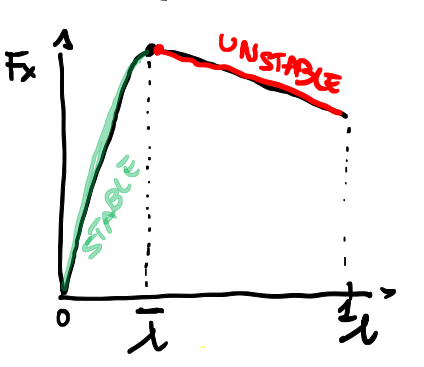
\includegraphics[width=0.5\textwidth]{lectures/2020-04-16/lambda-graph.png}
    \caption*{Relation between $\lambda$ and the breaking force.}
\end{figure}

\begin{figure}[H]
    \centering
    \begin{tikzpicture}[node distance=2.5cm,auto,>=latex']
        \node [int] (abs) {ABS algo};
        \node [sum] (sum) [left of=abs, node distance=2cm] {};
        \node (in) [left of=sum, node distance=2cm] {};
        \node [int] (sys) [right of=abs, node distance=3cm]{System};
        \node [coordinate] (split) [right of=sys, node distance=2cm]{};
        \node (end) [right of=sys, node distance=4cm]{};
        \node [int] (sws) [below of=sys, node distance=1cm]{SW-sensing};

        \draw[->] (in) edge node {$\overline{\lambda}$} (sum);
        \draw[->] (sum) edge node {} (abs);
        \draw[->] (abs) edge node {$u(t)$} (sys);
        \draw[->] (sys) edge node[pos=0.8] {$\lambda$} (end);
        \draw[->] (split) |- node {} (sws);
        \draw[->] (sws) -| node[pos=0.9] {$-$} (sum);
    \end{tikzpicture}
    \caption*{ABS system}
\end{figure}

The problem can be divided into subproblems:
\begin{itemize}
    \item Model of the system
    \item SW-estimation of $\lambda$ ($v$ is not directly measurable, so $\lambda$ cannot be computed)
    \item Design of the ABS control algorithm
\end{itemize}

Why black-box modelling?
The control variable $v$ (the voltage to the actuator) controls a complex systems from the actuator to $\lambda$.
The system can be seen as a chain of components:
\begin{itemize}
    \item Current dynamics and electric motor
    \item Position dynamics of the actuator
    \item Dynamics of the hydraulic circuit of the break system
    \item Tire dynamics
    \item Wheel rotational dynamics
    \item Vehicle full dynamics
\end{itemize}

White box (physical) modelling: write the equations from \emph{first principles}.

Black box modelling: experiment $\rightarrow$ collect data $\rightarrow$ build model.
Using only I/O measured data we can \emph{learn} a mathematical model of the I/O behavior of the system.

\chapter{Black-box non-parametric identification of I/O systems using state-space models}

\begin{figure}[H]
    \centering
    \begin{tikzpicture}[node distance=2.5cm,auto,>=latex']
        \node [int, ellipse] (sys) {system};
        \node (in) [left of=sys, node distance=2cm] {};
        \node (noise) [above of=sys, node distance=1.5cm] {};
        \node (end) [right of=sys, node distance=2cm]{};

        \draw[->] (in) edge node {$u(t)$} (sys);
        \draw[->,dotted] (noise) edge node {$d(t)$ \emph{(not measured disturbance)}} (sys);
        \draw[->] (sys) edge node {$y(t)$} (end);
    \end{tikzpicture}
\end{figure}

\textbf{Measured data}
\begin{align*}
    \left\{u(1), u(2), \ldots, u(N)\right\} &\quad \text{(input)} \\
    \left\{y(1), y(2), \ldots, y(N)\right\} &\quad \text{(output)}
\end{align*}

\begin{remark}[general path of a parametric identification methods]

\begin{enumerate}
    \item Collect data: $\left\{u(1), u(2), \ldots, u(N)\right\}$, $\left\{y(1), y(2), \ldots, y(N)\right\}$
    \item Select \textbf{a-priori} a class/family of parametric models: $\mathcal{M}(\theta)$
    \item Select \textbf{a-priori} a performance index (it gives an order to the quality of the models)
    \item Optimization step (minimize $J(\theta)$ w.r.t $\theta$): $\hat{\theta}_N = \argmin_\theta J(\theta)$ $\rightarrow$ optimal model $\mathcal{M}(\hat{\theta}_N)$
\end{enumerate}

$J(\theta): \RR^{n_\theta} \rightarrow \RR^+$ (where $n_\theta$ is the order of the model).

$\mathcal{M}(\theta_1)$ is better than $\mathcal{M}(\theta_2)$ if $J(\theta_1) < J(\theta_2)$.

\end{remark}

In this chapter we are presenting a totally different system identification approach: \textbf{not parametric}.
\begin{itemize}
    \item No a-priori model-class selection
    \item No performance index definition
    \item No optimization task
\end{itemize}

\section{Representations}

\subsection{Representation \#1: state-space}

\[
\begin{cases}
    x(t+1) = F x(t) + G u(t) & \qquad \text{state equations} \\
    y(t+1) = H x(t) + D u(t) & \qquad \text{output equations}
\end{cases}
\]

Where $F$, $G$, $H$ and $D$ are matricies defined as follows:
\begin{align*}
    F = \begin{bmatrix}
        \\
        n \times n \\
        \text{state matrix} \\ \\
    \end{bmatrix}
    &
    \qquad
    G = \begin{bmatrix}
        \\
        \\
        n \times 1 \\
        \text{input} \\
        \text{matrix} \\ \\
    \end{bmatrix}
    \\ \\
    H = \begin{bmatrix}
        1 \times n \;\;\; \text{output matrix}
    \end{bmatrix}
    &
    \qquad
    D = \begin{bmatrix}
        1 \times 1 \;\;\; \text{i/o matrix}
    \end{bmatrix}
\end{align*}

Assuming 1 input and 1 output, it can be extended for multiple inputs and outputs. Usually $D=0$ for \emph{strictly-proper systems}.

\begin{remark}[S.S representation is not unique]
    $F_1 = TFT^{-1}$, $G_1 = TG$, $H_1 = HT^{-1}$, $D_1 = D$ for any invertible matrix $T$. The system $\{F, G, H, D\}$ is equivalent to $\{F_1, G_1, H_1, D_1\}$.
\end{remark}

\begin{example}
    \[
        \begin{cases}
            x_1(t+1) = \frac{1}{2} x_1(t) + 2u(t) \\
            x_2(t+1) = x_1(t) + 2x_2(t) + u(t) \\
            y(t) = \frac{1}{4}x_1(t) + \frac{1}{2}x_2(t)
        \end{cases}
    \]
    In this case $n=2$, $x(t) = \begin{bmatrix}
        x_1(t) \\
        x_2(t)
    \end{bmatrix}$, one input $u(t)$ and one output $y(t)$.

    \begin{align*}
        F = \begin{bmatrix}
            \frac{1}{2} & 0 \\
            1 & 2
        \end{bmatrix}
        & \qquad
        G = \begin{bmatrix}
            2 \\ 1
        \end{bmatrix}
        \\
        H = \begin{bmatrix}
            \frac{1}{4} & \frac{1}{2}
        \end{bmatrix}
        & \qquad
        D = 0
    \end{align*}
\end{example}

\subsection{Representation \#2: transfer-function}

\[
    W(z) = \frac{B(z)}{A(z)} z^{-k} = \frac{b_0 + b_1z_{-1} + b_2z^{-2} + \ldots + b_pz^{-p}}{a_0 + a_1z^{-1} + a_2z^{-2} + \ldots + a_nz^{-n}} z^{-k}
\]

$W(z)$ is a rational function of the \emph{z} operator: it's a \emph{digital filter}.

It's very easy to move from T.F. representation to a time domain description of the system.

\begin{example}
    \begin{align*}
        & y(t) = \underbrace{\begin{bmatrix}
            \frac{1+\frac{1}{2}z^{-1}}{2+\frac{1}{3}z^{-1}+\frac{1}{4}z^{-2}} z^{-1}
        \end{bmatrix}}_{W(z)} u(t) \\
        & 2y(t) + \frac{1}{3}y(t-1) + \frac{1}{4}y(t-2) = u(t-1) + \frac{1}{2}u(t-2) \\
        & y(t) = \underbrace{-\frac{1}{6}y(t-1) - \frac{1}{8}y(t-2)}_\text{old values of $y(t)$} + \underbrace{\frac{1}{2}u(t-1) + \frac{1}{4}u(t-2)}_\text{old values of input}
    \end{align*}

\end{example}
\begin{remark}[Notational remark]
    $\displaystyle W(z) = \frac{z^{-1}}{1 + \frac{1}{3}z^{-1}}$ is called an IIR (\emph{Infinite Impulse Response}) filter.\\
    $\displaystyle W(z) = z^{-1} + \frac{1}{2}z^{-2} + \frac{1}{4}z^{-3}$ is called a FIR (\emph{Finite Impulse Response}) filter.
\end{remark}